\documentclass[UTF8,a4paper,11pt,fontset=fandol]{ctexart}
\usepackage[a4paper,top=2.3cm,bottom=2.3cm,left=2.5cm,right=2.5cm]{geometry}
\usepackage{amsmath,amssymb,booktabs,graphicx,float,xcolor,array,enumitem,hyperref,xurl,listings,caption}
\hypersetup{colorlinks=true,linkcolor=black,citecolor=black,urlcolor=blue}
\setlength{\parindent}{2em}
\linespread{1.25}
\renewcommand{\arraystretch}{1.2}
\setlist{nosep,leftmargin=2.5em}
\captionsetup{font=small,labelfont=bf}
\lstset{basicstyle=\ttfamily\small,breaklines=true,frame=single,columns=fullflexible}
\title{面向综合 AI 应用机会的多源智能挖掘与价值评估系统\\基于 B01 公开数据的探索性研究}
\author{}
\date{}

\begin{document}
\maketitle

\begin{abstract}
生成式人工智能应用快速扩展后，公开网络中同时存在用户需求、产品宣传、技术展示和内部开发记录。本文面向综合 AI 应用机会，构建从多源采集、清洗、机会判别、语义主题聚合、价值排序到决策支持的可追溯流程。B01 在 90 日窗口内从 GitHub、Hacker News、量子位、IT之家和 V2EX 获取公开记录，清洗后保留 2,561 条。系统以可观察需求、AI 核心性、技术可实现性和排除项组织机会判断，并将全量判断按用户授权登记为人工确认字段；其中 509 条材料完成逐条审阅，2,052 条采用已有 AI 判断转登记。全量结果包含 100 条机会记录，并形成 14 个主题，其中 12 个为单记录主题，轮廓系数为 0.204。针对 509 条逐条审阅子集，本文以五折嵌套交叉验证比较 TF-IDF 逻辑回归和 ComplementNB、冻结多语言 E5 向量上的逻辑回归和 RBF-SVM，以及内层选择参数的多层感知机（MLP）。字符 TF-IDF 逻辑回归平均精确率最高，为 $0.488\pm0.077$；RBF-SVM 平衡准确率最高，为 $0.720\pm0.054$。留一来源验证显示来源间表现差异明显，且部分来源正例不足以稳定估计。分类结果用于检查逐条审阅标签的复现情况，不外推为独立真人真值下的模型性能。结果支持对系统链路、模型选择和来源迁移边界的探索，不足以确认市场热点或行业需求占比。

\noindent\textbf{关键词：} AI 应用机会；多源采集；语义聚类；人工复核；机器学习；来源迁移
\end{abstract}

\section{引言}

\subsection{研究背景}

人工智能应用的进入门槛持续降低，公开网络中出现了大量与 AI、Agent、RAG 和自动化有关的项目、讨论及资讯。然而，记录中同时混有终端用户的求解诉求、开发者内部任务、产品介绍、新闻转述和营销表达。若将这些文本直接按出现频率或平台排序汇总，容易把技术热度误写成真实需求，把同一事件的转载误写成多源验证，也容易忽略正文不完整和热度指标缺失带来的不确定性。

赛题要求系统围绕给定需求方向完成多源采集清洗、机会判别与分类、主题聚合、价值评估和决策支持五项任务。其难点不在于生成一个单独的分类标签，而在于把原始来源、正文证据、机会条件、主题成员和价值分数串成可追溯链路。本文将这条链路作为研究对象，研究问题包括：如何在来源异质、内容完整度不同的情况下保留可解释的数据证据；如何用结构化机会条件区分需求与宣传；如何在确认边界不足时把模型输出与代理复核清晰分层；以及如何防止主题聚合和价值排序超出数据实际支持范围。

\subsection{研究内容与贡献}

本文的工作集中在以下三个方面。第一，设计了批次隔离的多源数据处理流程，保存原始字段、清洗记录、正文快照、去重关系和质量标记。第二，建立了带证据回溯的机会判别与分层复核流程。模型判断由可观察需求、AI 核心性、技术可实现性和排除项共同决定，复核结果区分原模型、可见标签辅助复核、盲复核和 AI 裁定，避免把模型标签写成真人真值。第三，构建语义主题和价值排序的探索性计算，并以审计指标明确主题稀疏、来源偏差和缺少人工评价时的结论边界。

本文不把 B01 公开数据当作所有平台的完整样本，也不把代理复核当作人工标注。论文的结论主要回答系统是否形成了可复现、可解释的机会发现流程，以及当前样本能支持哪些探索性观察。

研究问题据此分为三层：多源数据在怎样的保留条件下能够形成可审计的样本；结构化机会条件及多轮模型对照能揭示哪些判断边界；语义聚类和加权评分在何种情况下只适合作为人工筛选工具。本文将来源覆盖、内容质量和复核状态一起报告，使主题排序能够连回其样本范围。

\section{系统设计与研究方法}

\subsection{总体流程}

系统以一次需求方向对应一个独立批次。批次首先保存需求描述、关键词、时间窗和来源请求记录；采集结果随后进行来源链接规范化、内容清理、相关性筛选和重复识别。清洗记录以批次号和连续编号关联正文快照。机会判别覆盖清洗结果中的全部记录，机会记录才进入语义表示、主题聚合和价值评估。决策支持层提供来源追溯、主题成员查询和策划案所需的证据接口。

图~\ref{fig:pipeline} 给出 B01 各处理阶段的数量变化。最后一列表示进入主题计算的人工确认机会候选，不能解释为已验证的市场机会。

\begin{table}[H]
  \centering
  \small
  \caption{赛题任务与系统处理结果}
  \label{tab:tasks}
  \begin{tabular}{@{}>{\raggedright\arraybackslash}p{0.16\textwidth}>{\raggedright\arraybackslash}p{0.39\textwidth}>{\raggedright\arraybackslash}p{0.35\textwidth}@{}}
    \toprule
    任务 & B01 结果 & 证据边界 \\
    \midrule
    采集清洗 & 共 2561 条清洗记录 & 公开检索样本 \\
    机会判别 & 共 2561 条全量人工确认标签，100 条机会 & 509 条逐条审阅标签，其余按授权登记 \\
    主题聚合 & 共 14 个人工确认主题 & 12 个单记录主题 \\
    价值排序 & 最高分为 C2（85.76） & 仅供探索筛选 \\
    决策支持 & 复核工作台、主题优先级视图与 C2 策划案 & 浏览器截图仍需补齐 \\
    \bottomrule
  \end{tabular}
\end{table}

\begin{figure}[H]
  \centering
  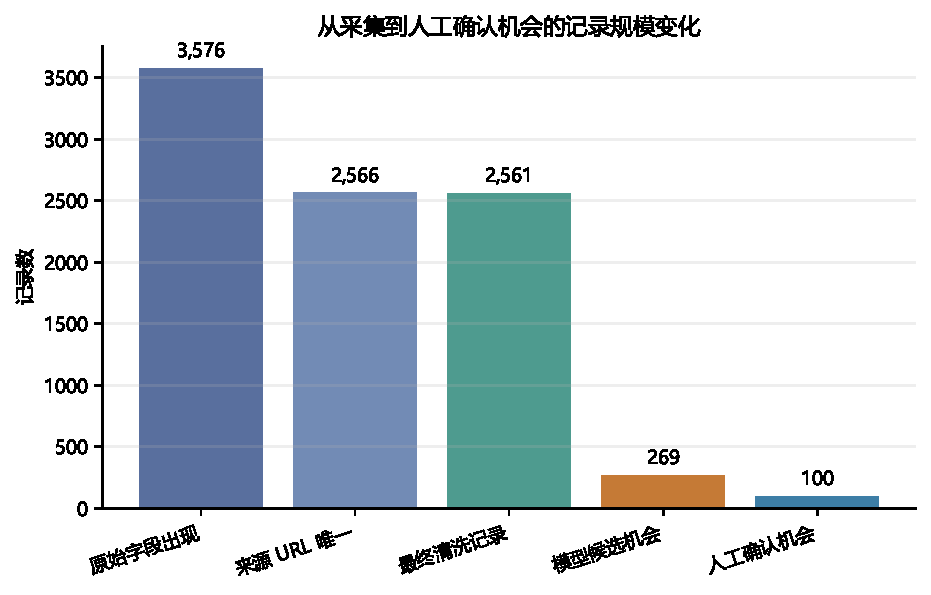
\includegraphics[width=0.92\textwidth]{../figures/fig02_pipeline_counts.pdf}
  \caption{B01 从采集到人工确认机会候选的记录规模。该图展示处理阶段计数，不表示采集召回率或分类准确率。}
  \label{fig:pipeline}
\end{figure}

为检查小样本条件下的神经网络分类是否改善机会标签复现，本文在人工确认样本上追加折外模型比较。该实验沿用结构化机会条件和分层复核边界，不改变全量自动判别结果。研究流程和证据关系如图~\ref{fig:method} 所示。

\begin{figure}[H]
  \centering
  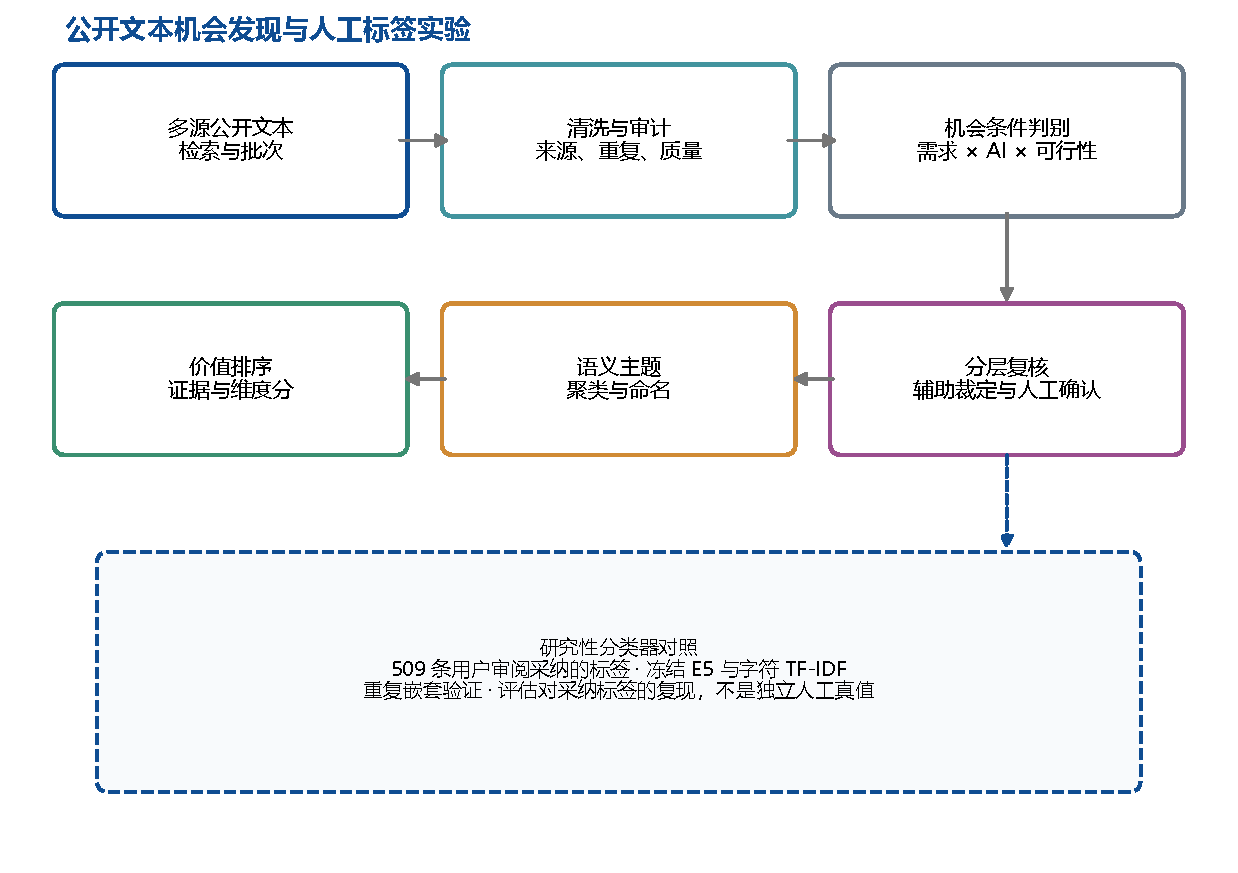
\includegraphics[width=0.98\textwidth]{../figures/fig15_opportunity_method.pdf}
  \caption{B01 机会发现流程与人工标签分类实验。下方模型比较评价对 509 条人工确认标签的复现能力。}
  \label{fig:method}
\end{figure}

\subsection{机会判别条件}

对记录 $i$ 定义四个布尔条件：$d_i$ 表示是否存在可观察的终端需求，$a_i$ 表示 AI 是否为解决路径的核心能力，$f_i$ 表示现有模型或成熟算法能否实现，$e_i$ 表示是否命中教程、科普、新闻、广告、融资宣传、开发者内部记录或测试任务等排除项。自动机会标签定义为

\begin{equation}
 y_i=d_i\land a_i\land f_i\land\neg e_i .
 \label{eq:opportunity}
\end{equation}

模型同时输出功能类别、行业类别、置信度、需求说明和正文证据。程序约束机会记录的功能和行业必须来自官方标签集合，并检查每条证据能在清洗后的正文中找到。非机会记录的两个分类字段保持为空。

\subsection{语义表示、聚类与价值评估}

主题聚合使用多语言文本向量表示标题和正文，采用 HDBSCAN 密度聚类。HDBSCAN 能在不同密度区域中识别簇并保留噪声点，相关方法见文献\cite{campello2013,mcinnes2017}。文本向量采用 multilingual-e5-small 的 384 维输出，模型使用 E5 技术报告所述的多语言文本嵌入路线\cite{reimers2019,e5report,e5model}。运行采用固定 revision、最长 512 个 token、attention-mask 均值池化和 L2 归一化，并以 ONNX Runtime CPU 推理。具体版本和量化文件随运行配置保存。在 B01 中，噪声记录不被删除，而是转为单记录主题。主题名称由模型根据代表成员和主题关键词生成，功能与行业使用成员标签的众数，仅作为候选描述。

主题 $c$ 的基础评分由三项维度组成：多源指向度 $S_c$、记录规模 $N_c$ 和互动信号 $H_c$。令 $s_c$ 为主题覆盖的不同网站数，$n_c$ 为主题记录数，则

\begin{equation}
 S_c=100\frac{s_c}{s_{\max}},\qquad
 N_c=100\frac{\log(1+n_c)}{\log(1+n_{\max})}.
 \label{eq:normalization}
\end{equation}

其中 $s_{\max}$ 和 $n_{\max}$ 分别为当前批次候选主题的最大网站覆盖数和最大记录数。互动信号先在来源与指标内部按对数尺度归一，再对主题成员中可用值求均值。综合分为

\begin{equation}
 V_c=0.45S_c+0.35N_c+0.20H_c .
 \label{eq:value}
\end{equation}

若某主题没有可用互动指标，互动维度不填零。设 $A_c$ 为主题 $c$ 的可用维度集合，则仅在集合内按 $\tilde w_{cj}=w_j/\sum_{k\in A_c}w_k$ 重新归一化权重。聚类质量用轮廓系数描述，其定义见 Rousseeuw 的聚类验证方法\cite{rouseeuw1987}；权重扰动通过 Kendall 秩相关系数\cite{kendall1938}进行敏感性描述，但不将排序稳定性解释为机会判断正确性。

\subsection{展示、权限与策划案边界}

第五项任务的展示层由两个角色组成。复核员可以查看逐条正文、来源证据和模型字段，并写入人工复核字段；决策者只能查看主题、成员数量、来源覆盖、维度分和优先级，不能通过决策视图读取逐条正文。接口在本地账号未配置时仅允许回环地址访问，配置账号后使用 HTTP Basic 认证区分角色。

当前实现已经覆盖批次选择、复核队列、正文证据查看和主题优先级查询。C2 策划案采用证据约束的文档输出：目标用户、痛点、功能和技术路线只能引用已保留的主题成员与来源，不从标题推断未观察到的业务事实。B01 的 C2 已形成可提交的策划案草稿，仍需通过真实用户访谈和试点验证。

\section{数据采集与预处理}

\subsection{数据来源与采集范围}

在本文中，B01 是本项目首个独立数据批次的内部编号，需求方向为综合 AI 应用机会，覆盖多个行业。时间窗为 2026 年 8 月 10 日 00:00 至 11 月 7 日 23:38:19（北京时间）。系统使用 GitHub REST 搜索仓库与 Issue\cite{githubapi}，使用 Hacker News Algolia 搜索 API\cite{hnapi}，使用量子位公开 WordPress 接口\cite{wpapi}，以及 IT之家和 V2EX 的公开订阅入口。不同来源提供的信号不同：GitHub 更接近工程能力和使用障碍，Hacker News 包含寻解讨论，资讯站提供应用和技术内容，V2EX 提供中文用户问题与工具讨论。

五个来源的记录规模如图~\ref{fig:sources} 所示。Hacker News 的记录数远高于其余来源，这一结构差异会影响后续主题规模和互动信号。GitHub 检索按星标与讨论排序，Hacker News 搜索按接口排序截取分页，量子位覆盖时间窗内接口返回的全部文章，IT之家与 V2EX 只返回当前订阅页内容。网站数量和采集记录数因此只描述本批次实际覆盖，不能换算成各行业用户需求比例。

\begin{figure}[H]
  \centering
  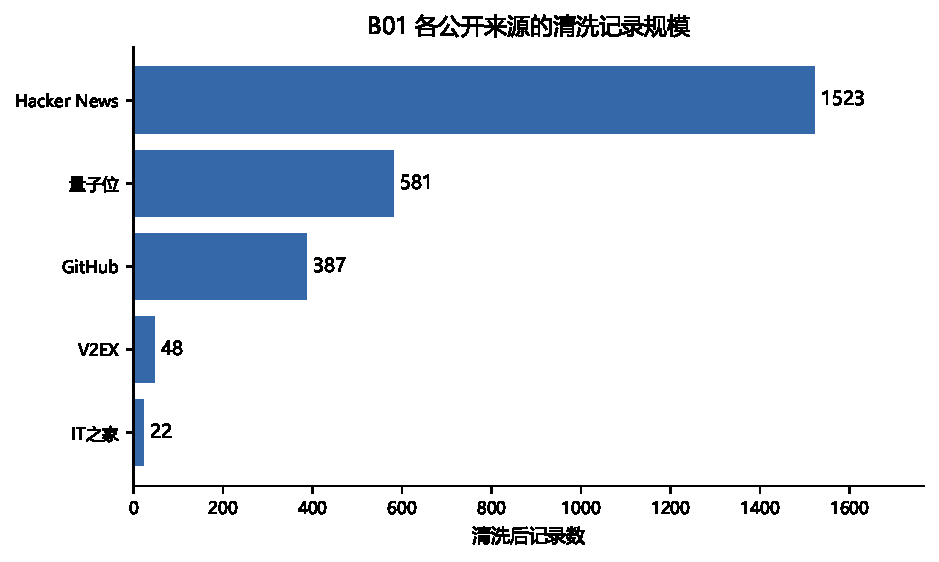
\includegraphics[width=0.86\textwidth]{../figures/fig01_source_counts.pdf}
  \caption{B01 清洗记录的来源规模。Hacker News 占比较高，来源结构存在明显偏斜。}
  \label{fig:sources}
\end{figure}

采集阶段共出现 3,576 次原始字段记录，其中同一来源记录可能因命中多个检索条件而重复。方向筛选排除 742 次字段出现，URL 归并排除 267 条，另有 1 条超出时间窗；得到 2,566 条来源 URL 唯一记录。再按正文证据归并 5 组完全或高度相似内容后，最终保留 2,561 条。来源数量分别为 Hacker News 1,523、量子位 581、GitHub 387、V2EX 48 和 IT之家 22。量子位接口在时间窗内返回的 723 篇记录均已获取；Hacker News、GitHub 搜索和 RSS 入口存在分页或历史覆盖限制，因此本文只把 B01 描述为公开样本批次，不外推平台总体分布。时间覆盖和来源信号的处理也遵循公开指标构造与阶段识别研究中强调的可计算规则\cite{song2020urban}。

\subsection{清洗、去重与质量标记}

清洗过程先对 URL 去除常见追踪参数，再进行 HTML 转文本、Unicode 规范化、空白清理和明显个人信息格式脱敏。重复处理分为同来源 URL 归并、完全相同正文识别和长正文近重复识别；近重复候选使用四字符 TF-IDF 与 shingle Jaccard 联合判断，采用的相似度阈值分别为余弦距离不高于 0.025 和 Jaccard 不低于 0.95\cite{salton1988}。被归并记录仍保留各自来源关系、平台 ID 和热度字段，跨平台指标不相加。该做法延续词项加权用于文本检索与相似性计算的基本思路\cite{salton1988}，但阈值由本批次清洗审计规则固定。

清洗结果中有 670 条内容被标记为不完整，495 条为短文本，907 条没有可用互动指标。图~\ref{fig:quality} 展示这些质量标记；一个记录可能同时命中多个标记。标题、简介和仅标题记录仍保留在数据集中，但在后续机会判别中不允许根据缺失正文外推业务事实。

\begin{figure}[H]
  \centering
  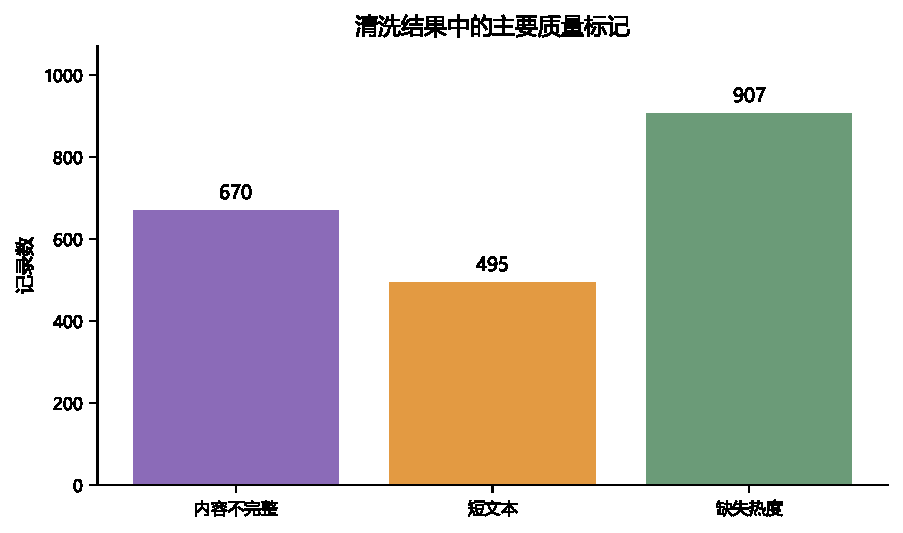
\includegraphics[width=0.82\textwidth]{../figures/fig03_quality_flags.pdf}
  \caption{清洗结果的主要质量标记。一个记录可以同时具有多个标记。}
  \label{fig:quality}
\end{figure}

数据质量审计逐条检查批次号、连续编号、来源链接、时间边界、正文路径、字符数和原始字段关联，JSONL、CSV 与正文快照的记录数均为 2,561。该审计证明处理关系一致，不证明内容相关性或机会标签质量。

采集阶段正文类型包括 \texttt{body} 类型记录 1,796 条、仅标题 396 条、项目简介 274 条、订阅正文 70 条和 README 25 条。\texttt{body} 是采集字段类型，不等同于每条记录都具备完整正文。近重复候选只对足够长的正文进行比较，标题与短文本不因语义相似而自动合并。个人信息清理基于邮箱、电话、IP 和用户名格式识别，无法覆盖所有自然语言线索；因此正文快照保存在本地，公开引用仍以原始来源链接为准。

图~\ref{fig:weekly-sources} 按发布周展示来源记录覆盖，便于区分持续覆盖和单周集中返回。最后一组覆盖至 11 月 7 日，为不完整自然周；Hacker News 的记录量整体较大，资讯与订阅来源的时间分布则受接口历史覆盖范围限制。该图报告的是本批次采集记录，不表示来源平台的实际发帖量。

\begin{figure}[H]
  \centering
  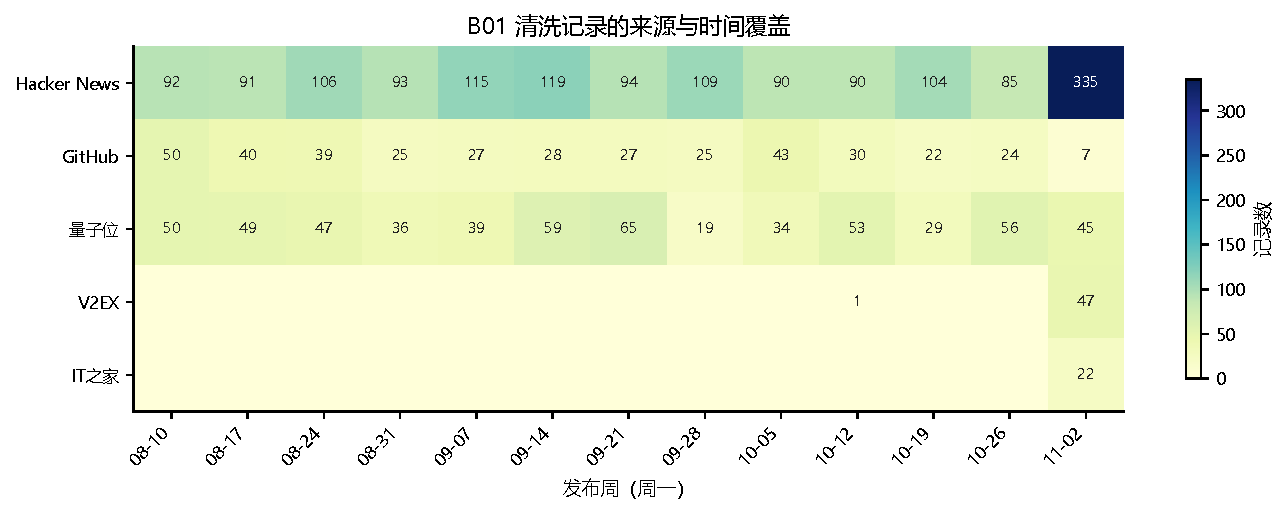
\includegraphics[width=0.98\textwidth]{../figures/fig07_weekly_source_heatmap.pdf}
  \caption{B01 清洗记录的来源与发布周分布。最后一组是截至 2026 年 11 月 7 日的不完整周，计数描述采集样本。}
  \label{fig:weekly-sources}
\end{figure}

不同来源的内容质量标记比例见图~\ref{fig:source-quality}。量子位、V2EX 和 IT 之家记录中热度字段缺失较多；GitHub 则有较高比例的简介型记录。各项比例以来源记录数为分母，缺失热度没有替换为零，质量标记也不会直接改写机会标签。

\begin{figure}[H]
  \centering
  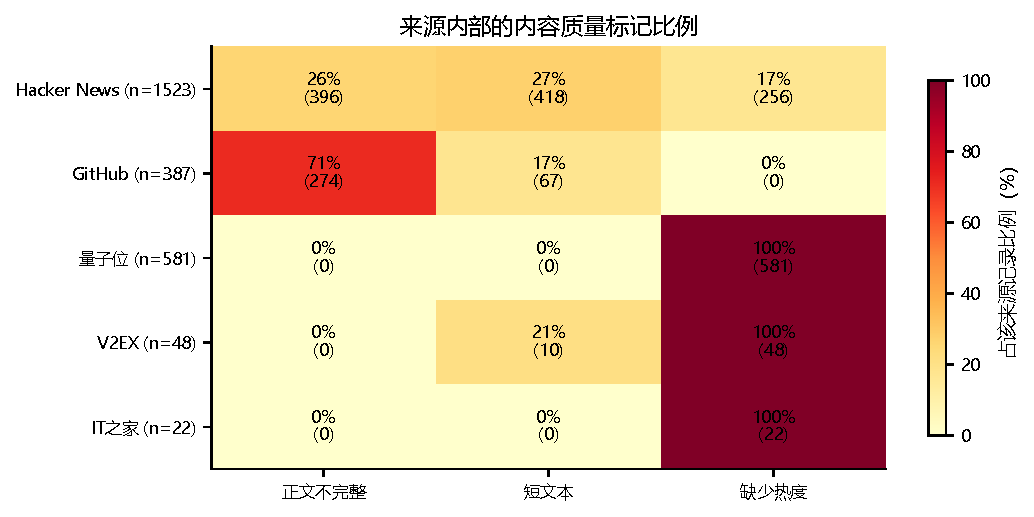
\includegraphics[width=0.88\textwidth]{../figures/fig08_source_quality_heatmap.pdf}
  \caption{来源内部的正文不完整、短文本和缺少热度比例；括号内为对应记录数。一个记录可同时命中多种质量标记。}
  \label{fig:source-quality}
\end{figure}

质量标记不直接改变机会标签；缺失的互动数据也不填为零。后续互动维度仅对实际可用的平台计数进行来源内归一化，以保留不同网站统计单位之间的差异。

\section{机会判别与人工复核}

\subsection{全量自动判别}

模型对 2,561 条清洗记录执行结构化判别，覆盖率为 100\%。原模型标记 269 条候选机会、2,292 条非机会。模型服务返回结构化结果，程序检查 record\_id 集合、标签合法性、机会逻辑和正文证据；全文中无法定位的证据会使批次重试。原模型累计使用 2,872,796 个输入 token 和 588,074 个输出 token，服务单价未配置，成本未知。

原模型的置信度是模型自评值，未进行概率校准。因而本文只把它用于筛选和流程计算，不将其写成已验证概率。

\subsection{分层复核队列}

复核队列包含全部 269 条模型候选机会，以及 240 条模型非机会样本。负例按来源网站和内容类型轮转，并在各层内优先选择模型置信度较低的记录。这样的设计适合查找模型边界和难例，但不是简单随机抽样，不能用来无偏估算 2,292 条模型非机会记录的整体漏判率。

图~\ref{fig:review-composition} 按来源和正文类型展示 509 条人工复核记录及其确认标签。复核样本中 Hacker News 占 282 条，GitHub 占 99 条；人工确认机会主要出现在 Hacker News 和量子位。该结构来自对原模型正例的全量纳入及定向负例抽样，不能解释为来源间机会率差异。

\begin{figure}[H]
  \centering
  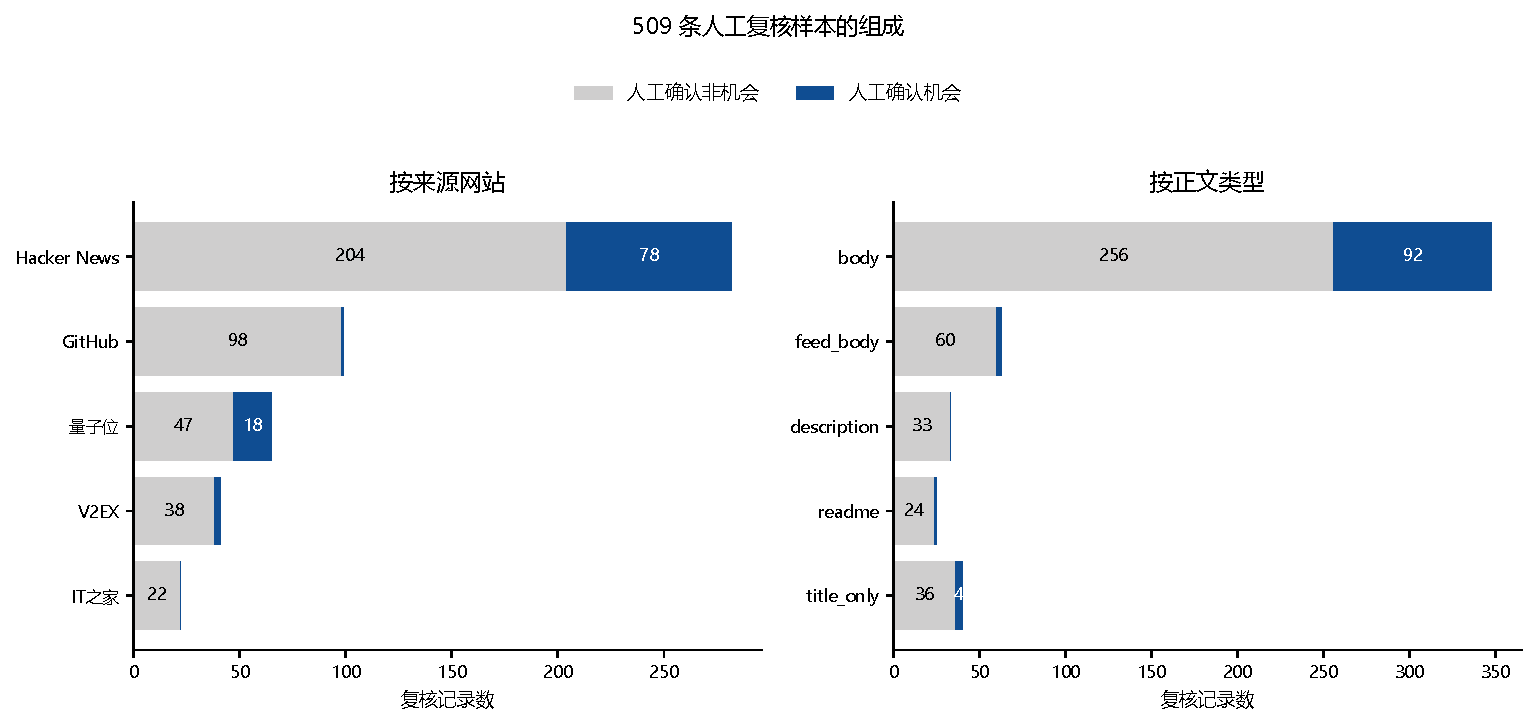
\includegraphics[width=0.98\textwidth]{../figures/fig09_review_sample_composition.pdf}
  \caption{509 条人工复核样本按来源网站和正文类型分组。颜色区分人工确认机会与人工确认非机会；样本构成为分层抽样结果。}
  \label{fig:review-composition}
\end{figure}

\subsection{可见标签、盲复核与 AI 裁定}

第一轮辅助复核同时提供正文和原模型字段；第二轮盲复核只提供记录文本和来源元数据。两轮都由同一模型完成，分别给出 141 条和 109 条机会判断；两轮判断一致 419 条，占 82.32\%。原模型与可见标签复核一致 379 条，与盲复核一致 337 条；三者同时一致 313 条，占 61.49\%。另有 328 条记录因判断分歧、边界标记或功能行业分类不一致进入再次裁定，这个集合不能等同于 328 条二分类分歧。

\begin{table}[H]
  \centering
  \caption{模型标签之间的一致记录数}
  \label{tab:review-agreement}
  \begin{tabular}{lrr}
    \toprule
    对照结果 & 一致记录数 & 占复核队列比例 \\
    \midrule
    可见标签辅助复核与盲复核 & 419 & 82.32\% \\
    原模型与可见标签辅助复核 & 379 & 74.46\% \\
    原模型与盲复核 & 337 & 66.21\% \\
    原模型、可见标签及盲复核三方一致 & 313 & 61.49\% \\
    \bottomrule
  \end{tabular}
\end{table}

表~\ref{tab:review-agreement} 中的比例衡量同一组模型输出之间的一致程度，不是准确率。由于所有判断均来自同一模型，输入提示及先前标签可能造成相关误差。

对这 328 条记录再次调用模型辅助裁定，并将 181 条稳定共识保留，形成覆盖 509 条队列的人工复核结果。其中 100 条为人工确认机会，占队列的 19.65\%；169 条相对原模型发生标签变化，占 33.20\%；160 条标记为边界情况。复核结果保留原模型标签、辅助复核结果和来源证据；用户随后阅读全部 509 条材料并确认对应分类，人工复核字段保存确认类别，备注为空。图~\ref{fig:labelshift} 展示人工确认标签相对原模型的变化。

\begin{figure}[H]
  \centering
  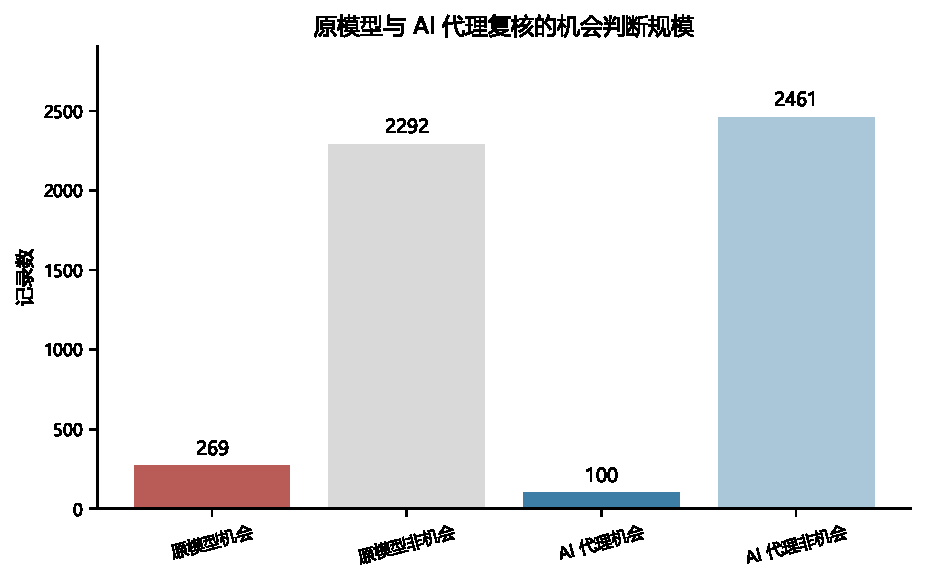
\includegraphics[width=0.82\textwidth]{../figures/fig04_label_shift.pdf}
  \caption{原模型与人工确认结果中的机会判断规模。全量结果包含 509 条人工复核标签及 2,052 条未复核原模型标签，因此该图不表示全量分类准确率。}
  \label{fig:labelshift}
\end{figure}

\subsection{面向人工复核标签的文本分类比较}

为比较小样本条件下不同文本模型对人工复核标签的复现能力，本文纳入 509 条记录，其中 100 条机会、409 条非机会。输入文本由标题与正文拼接，并截取至 12,000 个字符。模型包括字符 2--5 gram TF-IDF 逻辑回归和 ComplementNB，以及多语言 E5 冻结向量上的逻辑回归、RBF-SVM 和 MLP。TF-IDF 在每个训练折拟合，最低词频为 2，最多保留 50,000 个特征，并采用子线性词频缩放与 0.98 的文档频率上限。逻辑回归使用 $C=1$；ComplementNB 使用 $\alpha=1$ 和归一化；RBF-SVM 使用 $C=1$、尺度自适应核参数及三折 sigmoid 校准。

E5 使用固定 revision 的 multilingual-e5-small，将输入截断至 512 个 token，输出 384 维向量，经注意力掩码均值池化和 L2 归一化。每个外层训练折单独拟合标准化器。MLP 隐藏单元候选为 8 或 16，正则化系数为 0.1 或 1.0；三折内层验证按平均精确率选参，学习率为 0.001，最多迭代 1,000 次，并采用平衡样本权重。所有模型使用外层五折交叉验证并重复两次；外层随机种子为 20261119。类别权重或平衡样本权重仅应用于训练数据。阈值 0.5 下报告 Macro-F1 与平衡准确率，同时报告平均精确率、ROC-AUC 及外层折间标准差。该标准差描述折间变异，不是置信区间。人工确认机会占 19.65\%，因此主要关注对类别不平衡较稳健的平均精确率。

表~\ref{tab:proxy-classifiers} 给出 10 个外层折的均值与标准差。字符 TF-IDF 逻辑回归的平均精确率最高，为 0.488；在冻结 E5 表示上，RBF-SVM 与 MLP 均高于 E5 逻辑回归。RBF-SVM 的平衡准确率为 0.720，是五种方法中的最高值。MLP 所有内外层拟合均收敛。不同指标的模型排序并不相同，当前样本不足以支持某一种方法普遍更优的结论。

\begin{table}[H]
  \centering
  \small
  \caption{人工复核标签上的嵌套交叉验证比较}
  \label{tab:proxy-classifiers}
  \begin{tabular}{lrrr}
    \toprule
    方法 & 平均精确率 & Macro-F1 & 平衡准确率 \\
    \midrule
    字符 TF-IDF + 逻辑回归 & $0.488\pm0.077$ & $0.661\pm0.036$ & $0.679\pm0.044$ \\
    字符 TF-IDF + ComplementNB & $0.459\pm0.089$ & $0.464\pm0.056$ & $0.648\pm0.061$ \\
    冻结 E5 + 逻辑回归 & $0.367\pm0.056$ & $0.614\pm0.056$ & $0.632\pm0.059$ \\
    冻结 E5 + RBF-SVM & $0.445\pm0.055$ & $0.660\pm0.049$ & $0.720\pm0.054$ \\
    冻结 E5 + 内层选择 MLP & $0.441\pm0.064$ & $0.643\pm0.034$ & $0.644\pm0.037$ \\
    \bottomrule
  \end{tabular}
\end{table}

图~\ref{fig:proxy-comparison} 汇总三种主要方法的折间指标，图~\ref{fig:classifier-family} 展示五种模型族的平均精确率与 ROC-AUC。图~\ref{fig:proxy-oof} 展示字符 TF-IDF、冻结 E5 逻辑回归和 MLP 的折外平均精确率—召回率曲线与阈值 0.5 混淆矩阵。这三种方法分别在 51、49 和 44 条记录上正确复现人工确认机会；该数量只比较复核样本，不代表全批次机会数量。

\begin{figure}[H]
  \centering
  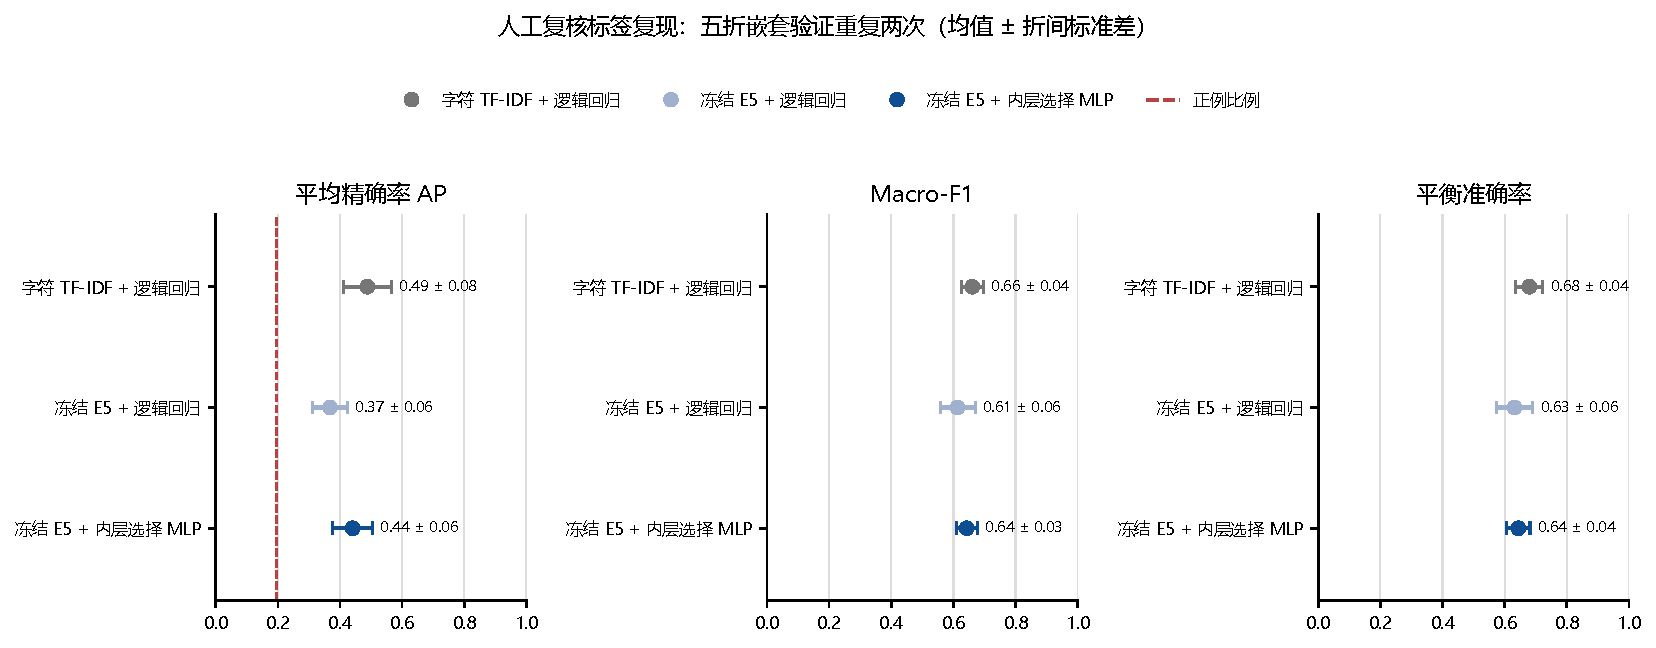
\includegraphics[width=0.98\textwidth]{../figures/fig10_proxy_classifier_comparison.pdf}
  \caption{509 条人工复核记录的重复五折外层交叉验证结果。点和误差线表示 10 个外层折的均值与标准差；红色虚线为复核样本机会比例。误差线不是置信区间。}
  \label{fig:proxy-comparison}
\end{figure}

\begin{figure}[H]
  \centering
  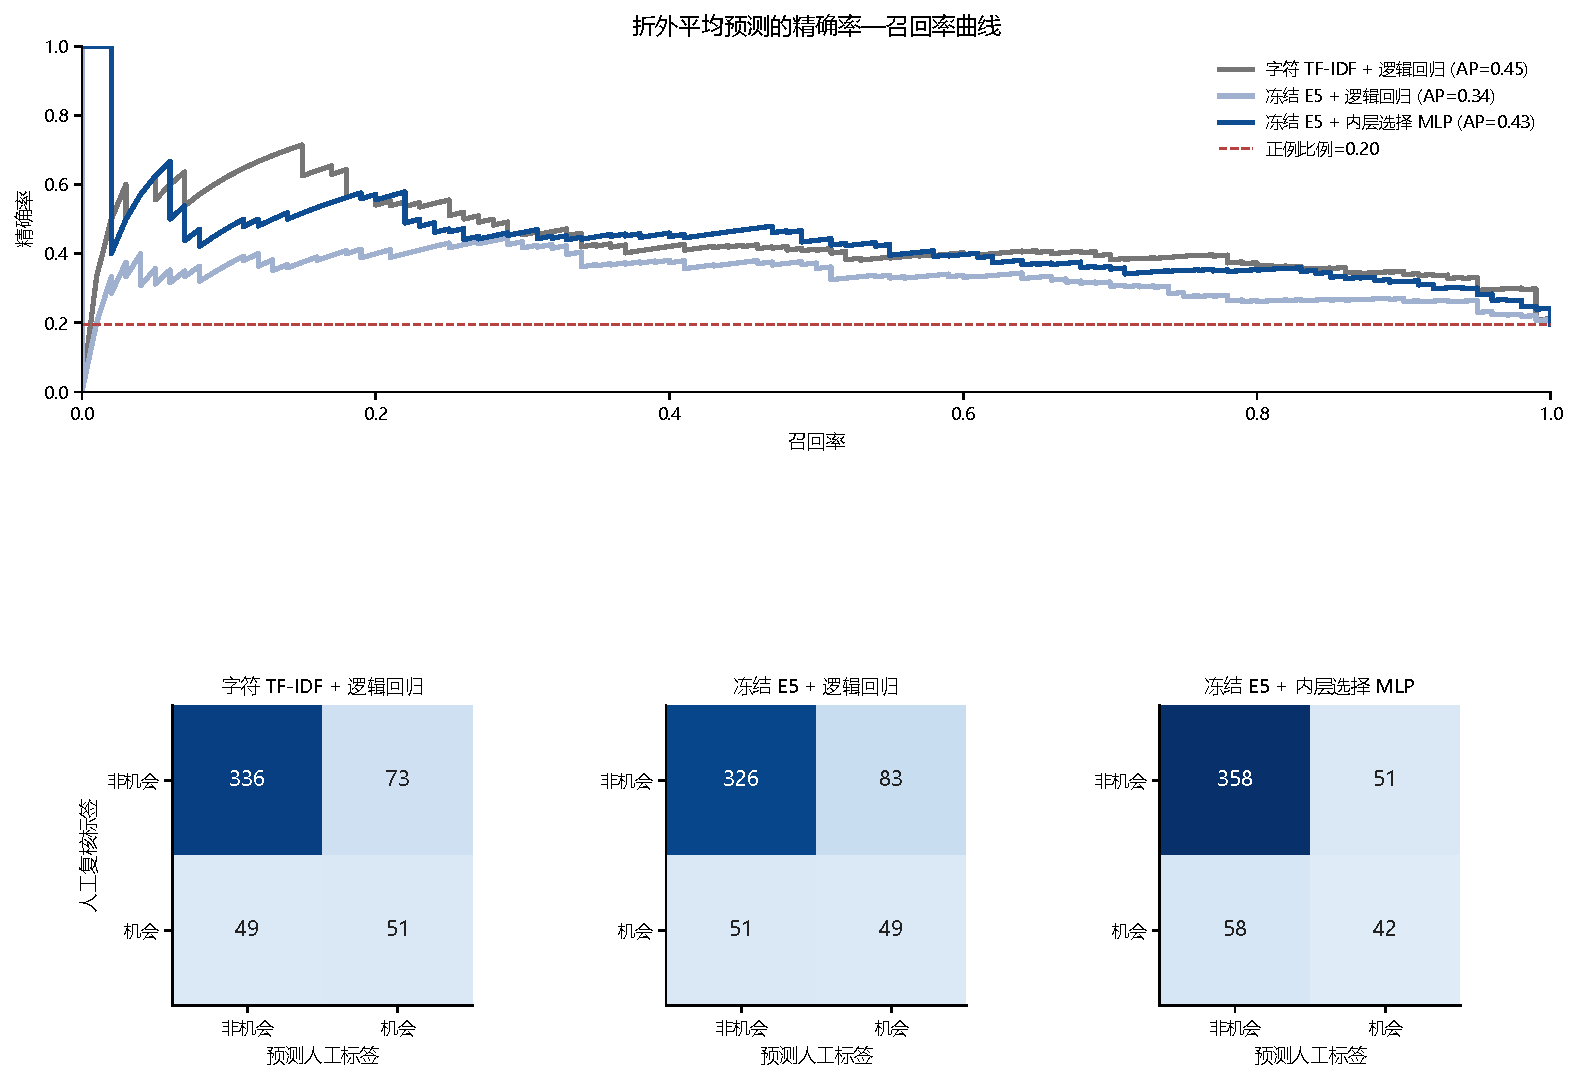
\includegraphics[width=0.98\textwidth]{../figures/fig11_proxy_classifier_oof.pdf}
  \caption{外层折外平均概率的精确率—召回率曲线及混淆矩阵。图中参照标签来自人工复核；结果不外推到未复核记录。}
  \label{fig:proxy-oof}
\end{figure}

\begin{figure}[H]
  \centering
  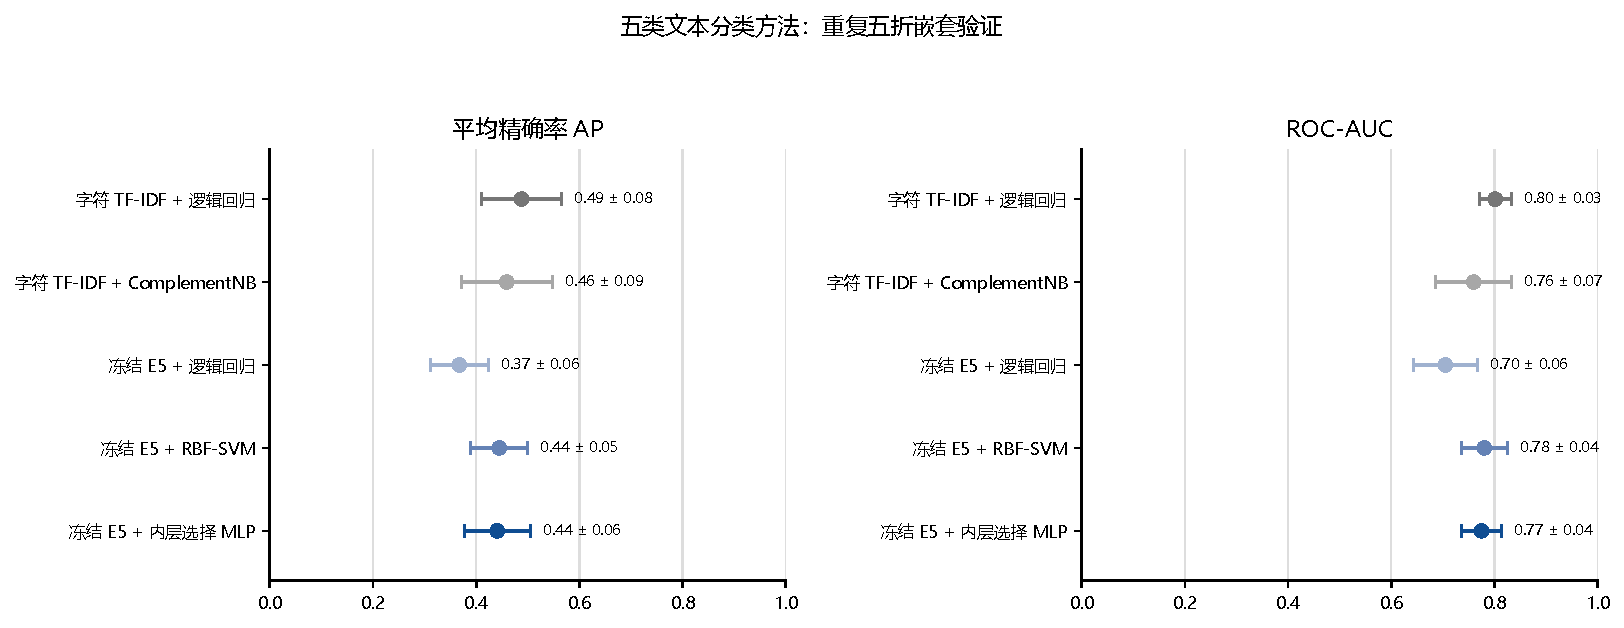
\includegraphics[width=0.98\textwidth]{../figures/fig16_classifier_family.pdf}
  \caption{五种模型族在人工复核标签上的重复嵌套验证结果。误差线为外层折间标准差；E5-RBF-SVM 经外层训练集内的 sigmoid 校准。}
  \label{fig:classifier-family}
\end{figure}

图~\ref{fig:embedding-pca} 将复核样本的 E5 向量压缩至两个主成分。两类标签在二维投影中明显交叠，且该投影仅解释向量总方差的 22.2\%；它用于观察表示空间结构，不作为分类边界或簇质量的检验。

为考察跨来源迁移，另进行留一来源验证：每次将一个网站的复核记录整体留作测试，其余四个来源用于训练，MLP 参数在训练来源内单独选择。五个来源的机会正例数量分别为 Hacker News 78 条、GitHub 1 条、量子位 18 条、V2EX 3 条和 IT 之家 0 条；因此 IT 之家留出时平均精确率与 ROC-AUC 不可估，其余来源的指标也受正例数稀少限制。图~\ref{fig:source-holdout} 报告三个主要模型的来源留出平均精确率，展示跨来源变化，不把这些小组样本分数合并为单一泛化估计。

\begin{figure}[H]
  \centering
  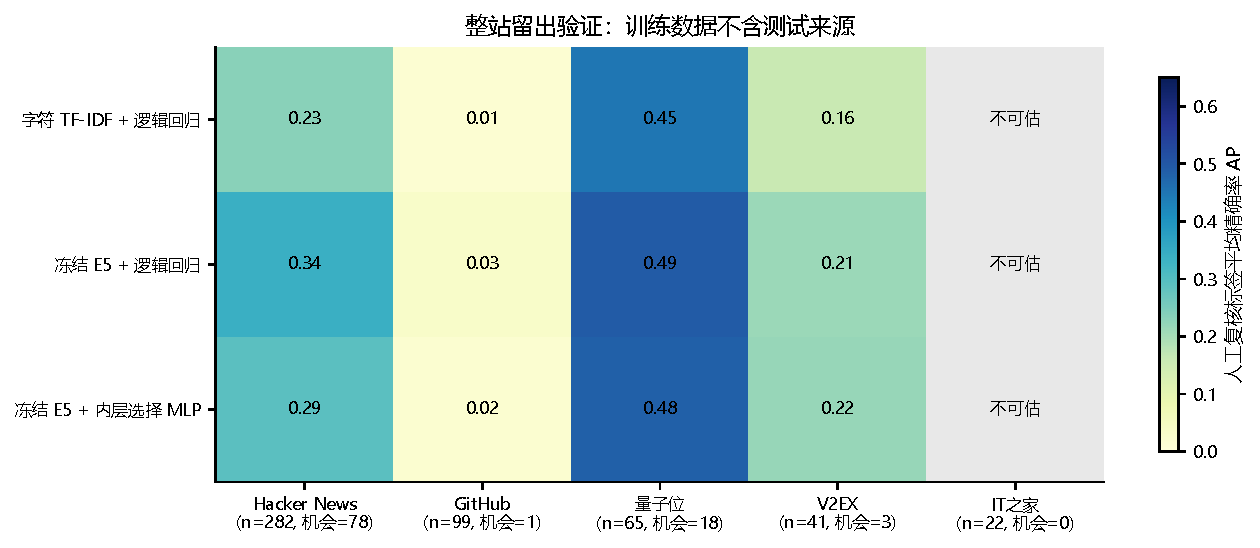
\includegraphics[width=0.98\textwidth]{../figures/fig17_source_holdout.pdf}
  \caption{留一来源验证的人工复核标签平均精确率。横轴同时列出留出来源的样本数和人工确认机会数；无正例来源不计算平均精确率。各来源正例数偏少，图中分数用于显示迁移差异。}
  \label{fig:source-holdout}
\end{figure}

\begin{figure}[H]
  \centering
  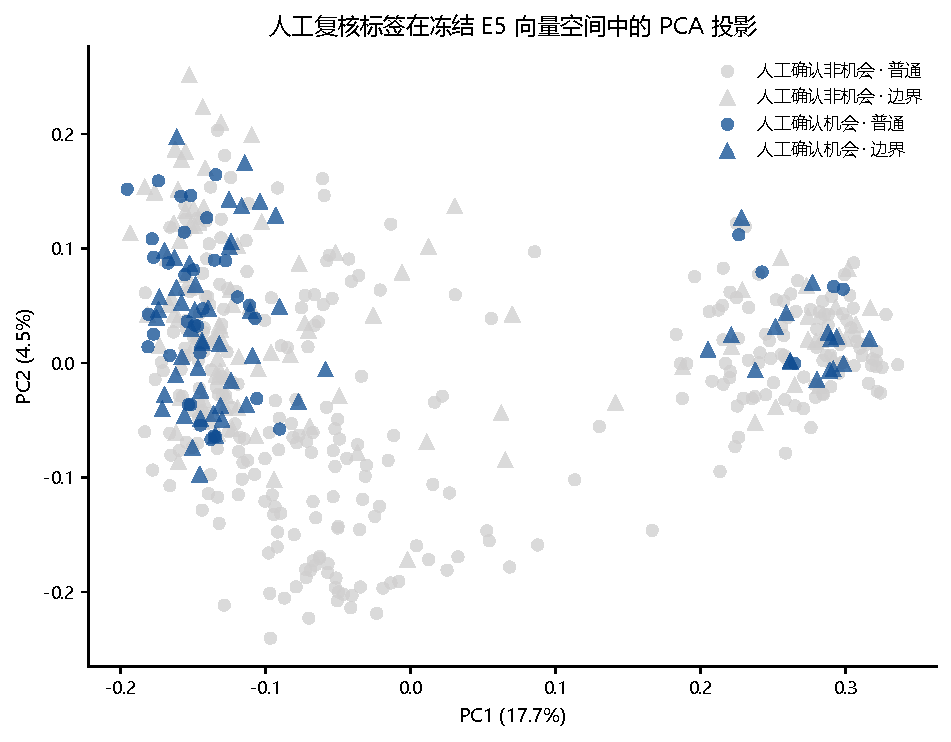
\includegraphics[width=0.76\textwidth]{../figures/fig12_embedding_pca.pdf}
  \caption{人工复核样本在冻结 E5 向量空间的 PCA 投影。符号区分被标记为边界的记录，颜色表示人工确认标签。}
  \label{fig:embedding-pca}
\end{figure}

该比较使用 509 条人工确认标签。人工字段记录确认类别，备注为空；模型辅助复核过程保留在 AI 使用记录中。复核队列的负例经过定向抽样，未进入队列的 2,052 条记录仍沿用原模型标签。因此交叉验证只描述人工复核样本，不能外推到全量记录。

\section{主题聚合与价值评估结果}

人工确认结果中 100 条机会记录进入语义聚合。使用 384 维多语言 E5 向量和 HDBSCAN，距离度量为欧氏距离，参数为 $\text{min\_cluster\_size}=5$、$\text{min\_samples}=2$。聚类得到 14 个主题，12 个主题只有一条记录，12 条噪声记录按单记录主题保留；轮廓系数在非噪声成员上计算，为 0.204。图~\ref{fig:topicscore} 对比各主题的成员规模与价值分，显示结果由两个较大的主题和 12 个单记录主题构成。

主题稀疏说明人工确认机会中仍有较多具体而分散的需求，不能把每个主题都视为成熟市场方向。排序第一的主题为 C2，价值分为 85.76，成员来自 GitHub、V2EX 和量子位；但该主题同时包含 AI 信息整理、游戏、医疗协同、Agent 平台和工具介绍等内容，主题内部异质性明显。因此 C2 在本文中仅作为系统发现的高分候选和聚类局限示例，不被解释为单一可立即立项的产品方向。

\begin{figure}[H]
  \centering
  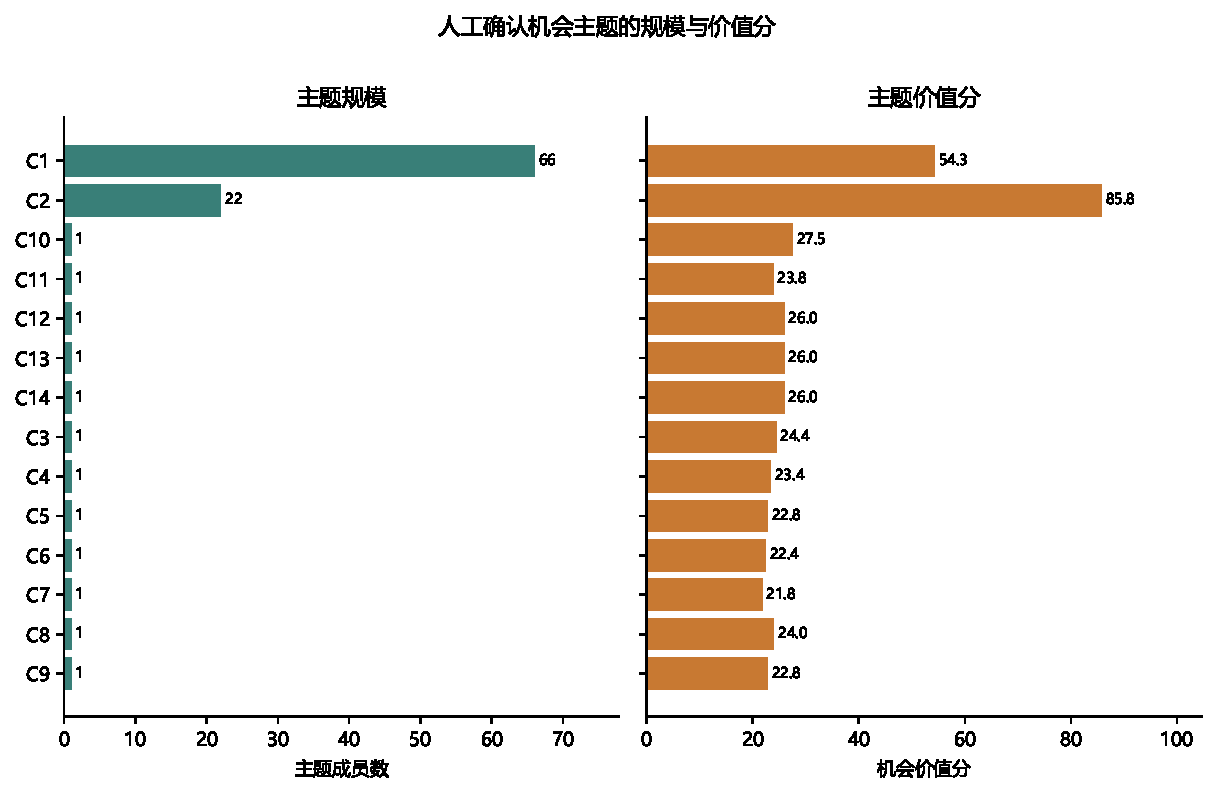
\includegraphics[width=0.95\textwidth]{../figures/fig05_topic_size_score.pdf}
  \caption{人工确认机会主题的成员规模与价值分。大多数主题为单记录主题，C1 和 C2 的规模明显高于其余主题。}
  \label{fig:topicscore}
\end{figure}

价值评分使用多源指向度、记录规模和互动信号三项维度，权重分别为 0.45、0.35 和 0.20。权重扰动下，来源、规模和互动信号情景与基准排序的 Kendall 相关系数分别为 1.000、1.000 和 1.000。由于主题数量较少且大量主题为单记录，该结果只能说明当前候选样本中的排序对权重变化不敏感，不能说明排序具有外部有效性；敏感性分析没有覆盖机会标签和聚类参数的变化。

图~\ref{fig:topic-dimensions} 将每个主题的三个维度分别展示，互动信号缺失的主题单独留空。C2 的跨来源覆盖与互动信号得分较高，C1 则主要依靠记录规模维度；这使得总分能够分解回已取得的数据字段，但仍受人工复核样本和平台覆盖偏差影响。

\begin{table}[H]
  \centering
  \caption{两个多记录主题的价值评分构成}
  \label{tab:topic-scores}
  \begin{tabular}{lrrrrr}
    \toprule
    主题 & 记录数 & 网站数 & $S_c$ & $N_c$ & $H_c$ / 总分 \\
    \midrule
    C2 智能体多场景应用 & 22 & 3 & 100.00 & 74.57 & 73.30 / 85.76 \\
    C1 AI 编程助手工作流 & 66 & 1 & 33.33 & 100.00 & 21.32 / 54.26 \\
    \bottomrule
  \end{tabular}
\end{table}

C2 的高分主要来自 3 个网站覆盖和较强的互动信号；C1 虽然包含 66 条记录，却全部来自 Hacker News，跨来源维度较低。该对比说明评分会把来源多样性纳入排序，但不同来源并不等于独立需求，仍需回到来源事件和成员文本判断重复传播及真实问题。

\begin{figure}[H]
  \centering
  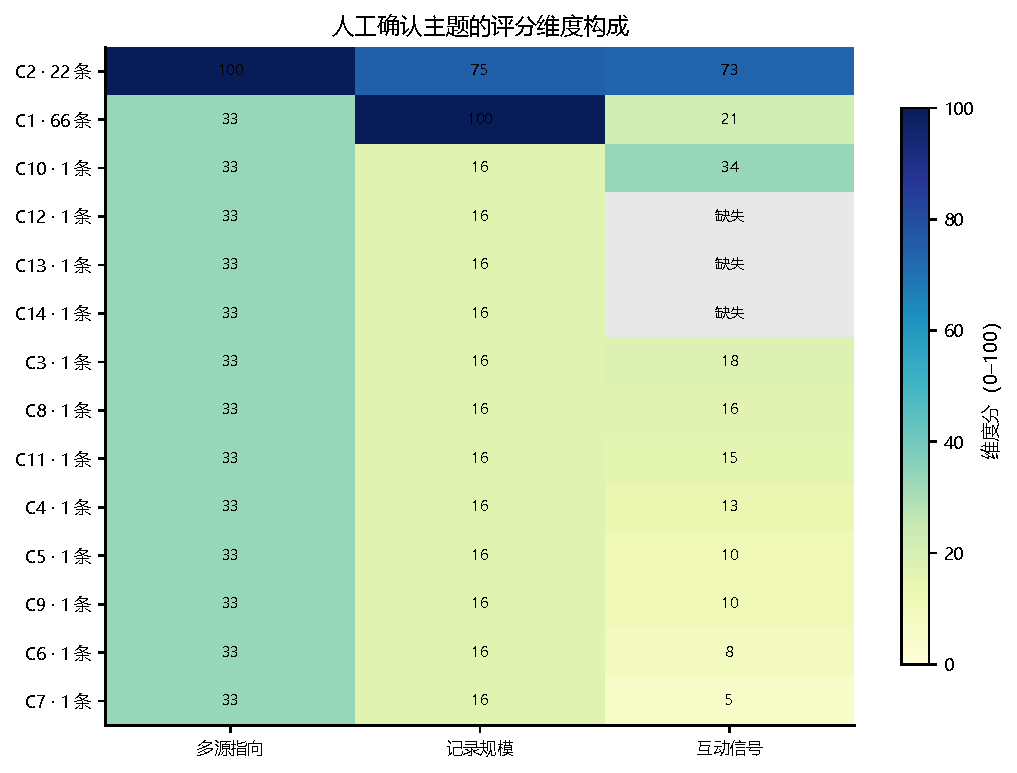
\includegraphics[width=0.77\textwidth]{../figures/fig13_topic_dimension_heatmap.pdf}
  \caption{14 个人工确认机会主题的多源指向度、记录规模和互动信号得分。互动信号缺失以空格显示，维度分仅用于当前 B01 候选排序。}
  \label{fig:topic-dimensions}
\end{figure}

为观察连续改变权重对排序的影响，图~\ref{fig:topic-rank-sensitivity} 从对称 Dirichlet$(1,1,1)$ 分布抽取 20,000 组权重，并对可用维度重新归一。点和误差线分别表示排名中位数及第 10--90 百分位，标签中的“前三”表示主题进入前三名的抽样比例。在这一权重先验下，C2 均保持前三，C1 有 91\% 的权重抽样进入前三。该比例描述指定权重扰动下的计算频率，不是主题真实优先级的概率；样本和机会标签的不确定性未包含在此模拟中。

\begin{figure}[H]
  \centering
  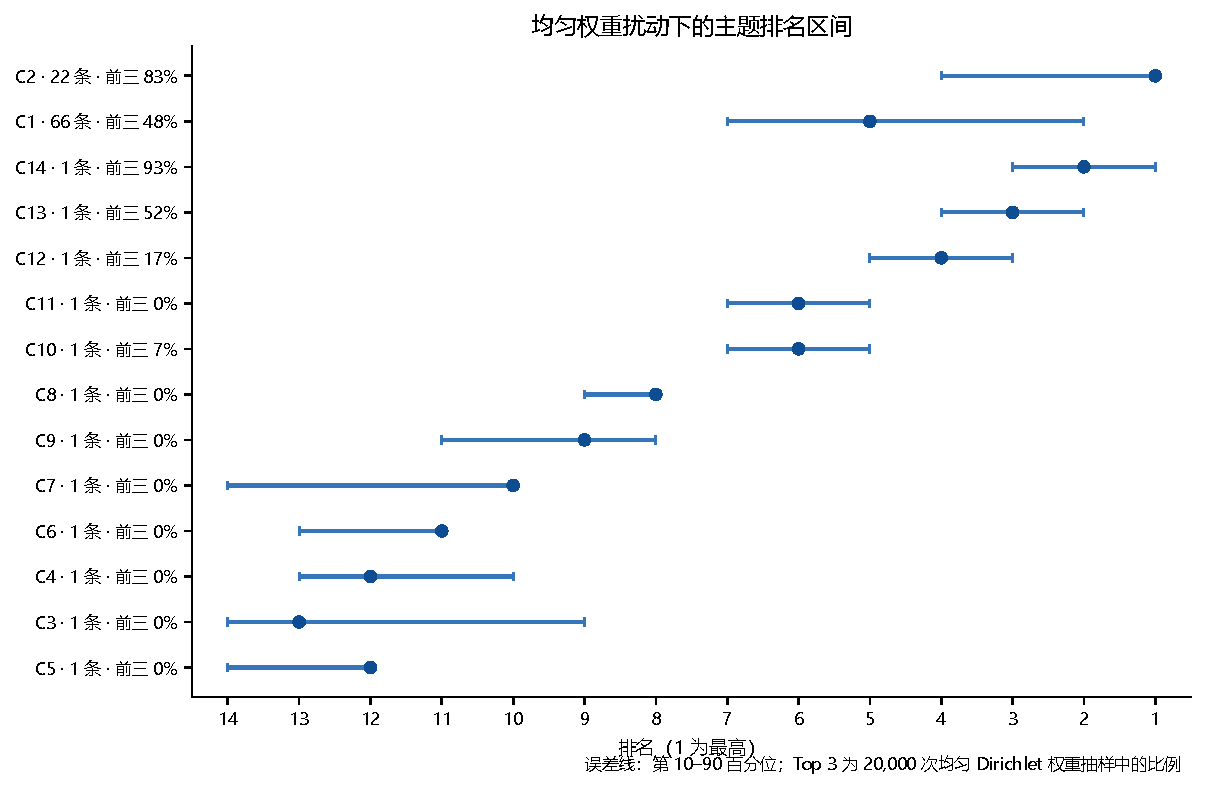
\includegraphics[width=0.86\textwidth]{../figures/fig14_topic_rank_sensitivity.pdf}
  \caption{人工确认主题在 20,000 组等先验权重抽样下的排名区间。误差线为第 10--90 百分位，“前三”比例只描述指定权重分布，不构成主题外部有效性证据。}
  \label{fig:topic-rank-sensitivity}
\end{figure}

\section{系统案例与讨论}

\subsection{从采集链路到决策支持}

本文的案例不是对某个产品已经成功落地的证明，而是展示系统如何把公开文本转成可追溯的决策候选。决策者可以先查看来源规模和正文质量，再查看代理复核中的原模型、盲复核和裁定差异，最后查看主题成员、来源覆盖和价值维度。这样的顺序把“记录是否构成机会”和“机会是否值得优先研究”分开，减少单一热度指标对决策的支配。图~\ref{fig:proxyconfusion} 展示全批次 2,561 条混合代理结果相对原模型的四类标签变化，其中 2,052 条未抽样记录沿用原标签。

\begin{figure}[H]
  \centering
  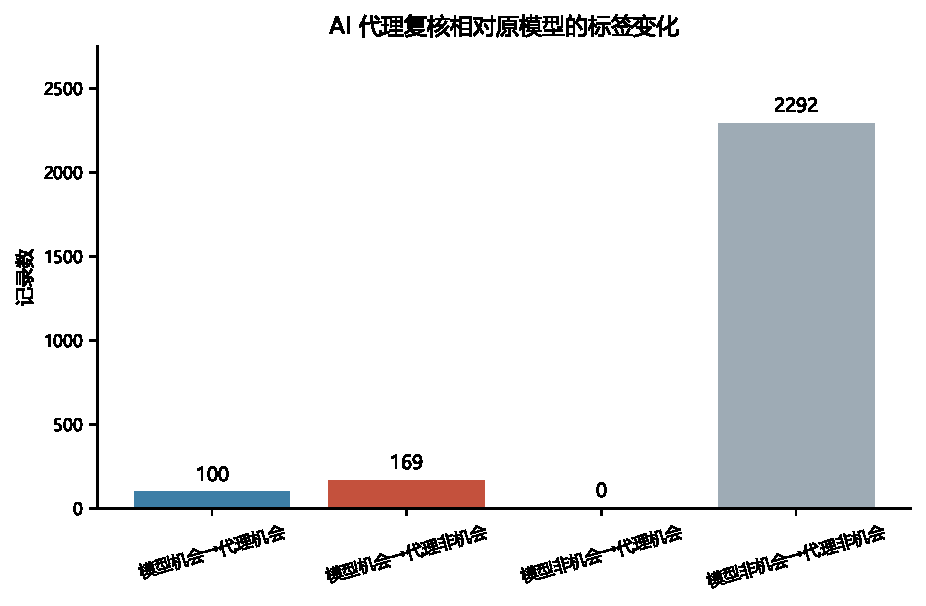
\includegraphics[width=0.82\textwidth]{../figures/fig06_proxy_confusion.pdf}
  \caption{混合代理结果相对原模型的标签交叉。四类共计 2,561 条；其中未抽样记录的标签沿用原模型，仅 509 条使用 AI 代理复核标签。}
  \label{fig:proxyconfusion}
\end{figure}

\subsection{数据与方法限制}

第一，来源之间的记录量和内容类型不均衡，Hacker News 占 B01 清洗记录的大部分，中文资讯和 RSS 历史覆盖有限。第二，部分记录只有标题、简介或短文本，907 条记录没有热度值，互动信号只能用于有数据的子集。第三，复核队列中的负例是面向难例的定向抽样，不能直接推断全量负例表现。第四，AI 代理裁定仍由同一模型完成，并且裁定输入包含此前模型输出，存在相关性与锚定风险。第五，主题轮廓系数较低、单记录主题较多，主题命名和功能行业众数不能替代人工主题边界判断。

因此，本文不报告经过人工真值验证的分类指标，也不把代理候选主题当成稳定市场热点。两轮复核与再次裁定均由同一 Codex 模型完成，结果只用于敏感性分析和系统链路验证，不能替代真人标注。正式比赛结果仍需要真人按统一标准确认至少全部预测机会记录，并对负例采用可解释的分层随机抽样，之后再生成正式 result2、result3 和 result4。系统已保留原始来源、处理配置、模型输出和代理裁定，能够在确认标签后重跑后续步骤。

\subsection{C2 候选方向的策划案框架}

C2 是当前代理评分最高的候选主题，包含 22 条记录，覆盖 GitHub、V2EX 和量子位三个来源，价值分为 85.76。成员标题涉及智能体架构、网络排障、医疗协同、代码模型和三维编辑等不同场景，因此 C2 的名称只能作为共同技术线索，不能直接等同于单一产品需求。

在证据边界内，C2 可形成待确认的策划案框架：目标是为需要多步骤知识检索、任务编排和结果回溯的团队提供可审计的智能体工作台；最小功能包括来源证据检索、任务分解与编排、过程日志、人工确认节点和结果引用；技术路线包括多语言向量检索、结构化模型调用、权限隔离与证据存储。上线前应以真人确认的需求记录为入口，比较引用正确率、任务完成时间和人工修改量，并对医疗等高风险场景单独设置人工审批。上述内容是由 C2 成员归纳出的实施假设，不是 B01 已观测到的用户承诺或产品效果。

\section{结论}

本文构建了一套面向综合 AI 应用机会的多源智能挖掘与价值评估系统，并在 B01 公开数据批次上完成了从采集、清洗、机会判别、代理复核、主题聚合到价值排序的可复现流程。系统保留了来源、正文、质量标记、模型证据、代理裁定和主题成员之间的处理关系，能够区分原模型标签、盲复核标签和 AI 代理标签。

B01 最终清洗得到 2,561 条记录。原模型覆盖全量记录并标记 269 条候选机会；509 条分层复核队列经过两轮辅助复核和冲突裁定后，形成 100 条 AI 代理机会候选。基于代理候选的语义聚合得到 14 个探索性主题，但其中 12 个为单记录主题，轮廓系数为 0.204。第五项任务已经实现复核工作台和决策者主题优先级视图，C2 策划案仍属于待确认框架。结果说明系统已经能够把复杂公开文本组织为可审计的候选链路，也同时暴露出来源偏差、正文缺失、定向抽样、模型相关性和主题稀疏等问题。

本文的主要结论是：在缺少真人真值时，完整记录处理链路和显式不确定性比输出一个看似精确的热点排名更重要。AI 代理结果可以用于系统调试、候选筛选和论文中的探索性案例，但不能替代人工真值，也不能支持准确率、召回率和外部市场占比等强结论。后续完成真人复核、分层随机评价和主题边界确认后，系统才能形成正式比赛结果和可执行的策划案。

因此，B01 的价值不在于证明某个 AI 方向已具备投资或上线条件，而在于展示从公开记录到决策候选的可核验处理过程。后续验证应先对全部原模型机会记录开展真人确认，再在非机会记录中按来源和正文完整度分层随机抽样；完成标签一致性检查后，重新计算主题、来源覆盖、价值分和排名稳定性。策划案的用户范围、功能优先级与风险控制也需由成员级原文和后续访谈确认。完成这些工作之前，C1 和 C2 仅能用于提出问题与安排验证，不能代表实际市场规模。

后续结果应继续保留批次、来源和标签版本，使人工确认后的正式结果能够与当前探索性结果逐项区分。

\begin{thebibliography}{99}
\bibitem{salton1988}
Salton G, Buckley C. Term-weighting approaches in automatic text retrieval[J]. Information Processing \& Management, 1988, 24(5): 513--523. DOI: \href{https://doi.org/10.1016/0306-4573(88)90021-0}{10.1016/0306-4573(88)90021-0}.

\bibitem{campello2013}
Campello R J G B, Moulavi D, Sander J. Density-based clustering based on hierarchical density estimates[M]//Pei J, Tseng V S, Cao L, et al. Advances in Knowledge Discovery and Data Mining. Berlin: Springer, 2013: 160--172. DOI: \href{https://doi.org/10.1007/978-3-642-37456-2_14}{10.1007/978-3-642-37456-2\_14}.

\bibitem{mcinnes2017}
McInnes L, Healy J, Astels S. hdbscan: Hierarchical density based clustering[J]. Journal of Open Source Software, 2017, 2(11): 205. DOI: \href{https://doi.org/10.21105/joss.00205}{10.21105/joss.00205}.

\bibitem{reimers2019}
Reimers N, Gurevych I. Sentence-BERT: Sentence embeddings using Siamese BERT-networks[C]//Proceedings of EMNLP-IJCNLP. 2019: 3982--3992. DOI: \href{https://doi.org/10.18653/v1/D19-1410}{10.18653/v1/D19-1410}.

\bibitem{e5report}
Wang L, Yang N, Huang X, et al. Multilingual E5 text embeddings: A technical report[EB/OL]. arXiv:2402.05672, 2024. \url{https://arxiv.org/abs/2402.05672}.

\bibitem{e5model}
intfloat. multilingual-e5-small[EB/OL]. Hugging Face. \url{https://huggingface.co/intfloat/multilingual-e5-small}.

\bibitem{rouseeuw1987}
Rousseeuw P J. Silhouettes: A graphical aid to the interpretation and validation of cluster analysis[J]. Journal of Computational and Applied Mathematics, 1987, 20: 53--65. DOI: \href{https://doi.org/10.1016/0377-0427(87)90125-7}{10.1016/0377-0427(87)90125-7}.

\bibitem{kendall1938}
Kendall M G. A new measure of rank correlation[J]. Biometrika, 1938, 30(1--2): 81--93. DOI: \href{https://doi.org/10.1093/biomet/30.1-2.81}{10.1093/biomet/30.1-2.81}.

\bibitem{githubapi}
GitHub. REST API documentation: Search[EB/OL]. \url{https://docs.github.com/en/rest/search/search}.

\bibitem{hnapi}
Algolia. Hacker News Search API[EB/OL]. \url{https://hn.algolia.com/api}.

\bibitem{wpapi}
WordPress. REST API Handbook[EB/OL]. \url{https://developer.wordpress.org/rest-api/}.
\end{thebibliography}

\section{复现说明}

本文代码按批次保存采集配置、清洗关系、模型输出、证据摘录和代理裁定。主要复现入口包括数据清洗审计、全量判别审计、代理结果审计和主题结果审计；具体命令、输入运行目录和依赖版本随项目说明及运行报告提供。

\end{document}
